% This file was created with tikzplotlib v0.10.1.
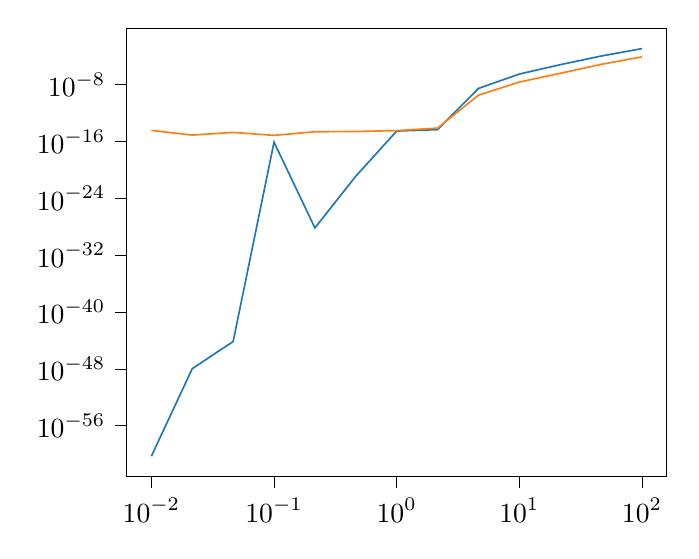
\begin{tikzpicture}

\definecolor{darkgray176}{RGB}{176,176,176}
\definecolor{darkorange25512714}{RGB}{255,127,14}
\definecolor{steelblue31119180}{RGB}{31,119,180}

\begin{axis}[
log basis x={10},
log basis y={10},
tick align=outside,
tick pos=left,
x grid style={darkgray176},
xmin=0.00630957329672048, xmax=158.489319423237,
xmode=log,
xtick style={color=black},
xtick={0.0001,0.001,0.01,0.1,1,10,100,1000,10000},
xticklabels={
  \(\displaystyle {10^{-4}}\),
  \(\displaystyle {10^{-3}}\),
  \(\displaystyle {10^{-2}}\),
  \(\displaystyle {10^{-1}}\),
  \(\displaystyle {10^{0}}\),
  \(\displaystyle {10^{1}}\),
  \(\displaystyle {10^{2}}\),
  \(\displaystyle {10^{3}}\),
  \(\displaystyle {10^{4}}\)
},
y grid style={darkgray176},
ymin=7.01737210775409e-64, ymax=0.874389456022799,
ymode=log,
ytick style={color=black},
ytick={1e-72,1e-64,1e-56,1e-48,1e-40,1e-32,1e-24,1e-16,1e-08,1,100000000},
yticklabels={
  \(\displaystyle {10^{-72}}\),
  \(\displaystyle {10^{-64}}\),
  \(\displaystyle {10^{-56}}\),
  \(\displaystyle {10^{-48}}\),
  \(\displaystyle {10^{-40}}\),
  \(\displaystyle {10^{-32}}\),
  \(\displaystyle {10^{-24}}\),
  \(\displaystyle {10^{-16}}\),
  \(\displaystyle {10^{-8}}\),
  \(\displaystyle {10^{0}}\),
  \(\displaystyle {10^{8}}\)
}
]
\addplot [semithick, steelblue31119180]
table {%
0.00999999977648258 5.17789406742998e-61
0.0215443465858698 1.07868330051655e-48
0.046415887773037 7.12027028429002e-45
0.100000001490116 8.09171463317758e-17
0.215443462133408 6.90843377314082e-29
0.464158892631531 1.30192029037409e-21
1 2.95530345680411e-15
2.15443468093872 4.66743790957096e-15
4.64158868789673 2.93215498115233e-09
10 3.10332432359728e-07
21.5443477630615 6.46061018468091e-06
46.4158897399902 0.000105934189037378
100 0.00118502157442826
};
\addplot [semithick, darkorange25512714]
table {%
0.00999999977648258 3.60787833692494e-15
0.0215443465858698 8.02530065746519e-16
0.046415887773037 1.89366486078451e-15
0.100000001490116 7.29376241898116e-16
0.215443462133408 2.34864413804607e-15
0.464158892631531 2.56312536041169e-15
1 3.42058140190921e-15
2.15443468093872 7.6518324195424e-15
4.64158868789673 3.28696022126687e-10
10 2.31944384735123e-08
21.5443477630615 3.96572569675992e-07
46.4158897399902 7.14922637485165e-06
100 8.22923942791689e-05
};
\end{axis}

\end{tikzpicture}
